% ---------------------------------------------------------------------------
% Evaluation (generated draft). Before compiling, check:
%  * citation keys: litinski2019game, zhu2026o3ls, silva2024multi, hofmeyr2026scheduling
%  * section labels: sec:composer, sec:layout, sec:model-supply,
%    sec:model-schedules, sec:hir-properties
% All figures and tables live in figures/evaluation/ and are produced by
% make_eval_plots.py from the rq/ results.
% ---------------------------------------------------------------------------
\section{Evaluation}
\label{sec:evaluation}

We evaluate Harvest at the logical patch level and answer five research questions.
RQ1 compares Harvest with four state-of-the-art lattice-surgery compilers (\S\ref{sec:eval-sota}).
RQ2 attributes the improvement to the individual stages of Harvest (\S\ref{sec:eval-contributions}).
RQ3 examines how much layout Harvest should schedule on and how much pruning recovers (\S\ref{sec:eval-provisioning}).
RQ4 evaluates the scheduler under different magic-state protocols (\S\ref{sec:eval-supply}).
RQ5 checks the validity of every schedule and measures the cost of compilation (\S\ref{sec:eval-validity}).

\subsection{Experimental Setup}
\label{sec:eval-setup}

\myparagraph{Benchmarks}
We use Clifford+T circuits from QASMBench (adders, multipliers, Ising models, neural-network circuits, $k$-nearest neighbors, swap tests, W states, and further small programs), QFT, QAOA, square Heisenberg models, random circuits, and VQE-UCCSD ansätze.
RQ1 uses \jannik{final count} 91 circuits with 2 to 98 logical qubits and 1 to 16{,}744 Pauli rotations (median 1{,}721).
RQ2--RQ5 use a subset of 47 circuits with 2 to 98 logical qubits.
\jannik{Update counts once the queued circuits with 64+ qubits and the large Ising instances finish.}

\myparagraph{Compilers}
We compare Harvest with four lattice-surgery compilers:
the fast-block layout and schedule of Litinski~\cite{litinski2019game},
O3LS~\cite{zhu2026o3ls},
earliest-available-first scheduling (EAF) by Silva et~al.~\cite{silva2024multi} on the blocks-of-four layout,
and PureMagic~\cite{hofmeyr2026scheduling}.
All compilers receive the same Pauli-rotation program produced by the Pauli graph composer (\S\ref{sec:composer}).
Unless stated otherwise, Harvest compiles each circuit on four layout templates, the ring, the blocks-of-four, and two dense templates (\S\ref{sec:layout}), and reports the template with the smallest space--time volume.
\jannik{Describe dense4 and dense4full in \S6.2.}

\myparagraph{Magic-state models}
RQ1 evaluates every compiler under two supply models.
Under \emph{instant} supply, every terminal always holds a magic state (the free model of \S\ref{sec:model-supply}), which isolates placement and routing.
Under \emph{cultivated} supply, a terminal receives a new magic state after a random delay with a mean of three logical timesteps; we average ten seeds per circuit.
RQ4 additionally uses distillation with fixed latency $\mu \in \{4, 10\}$ and two further cultivation variants.

\myparagraph{Metrics}
We report the number of logical timesteps $T$, i.e., the makespan of \S\ref{sec:model-schedules}, the area in patches, and the space--time volume $\text{area} \cdot T$.
To compare circuits of different size, we normalize by two lower bounds.
No schedule can be shorter than the critical path $T_{cp}$ of $G_O$, and no layout can hold fewer patches than the $n$ data patches of the program.
We therefore report $T/T_{cp}$, the area per logical qubit $\text{area}/n$, and the normalized volume $\text{Vol}/(n \cdot T_{cp})$, each of which is at least one.
Under cultivated supply, $T_{cp}$ remains a lower bound but is looser, since a tight bound also accounts for the magic-state supply of a layout (RQ4).
We aggregate over circuits by the geometric mean.

\myparagraph{Validation and hardware}
We replay every Harvest schedule through the validator of \S\ref{sec:hir-properties}, which checks (V1)--(V4) before and after pruning.
We run all experiments on \jannik{check machine} an AMD Ryzen~5 7000-series processor with 16\,GB of RAM under Ubuntu~24.04.

%% ---------------------------------------------------------------------------
\subsection{Comparison with the State of the Art}
\label{sec:eval-sota}

\researchquestion[RQ1: State of the art]{How does the space--time volume of Harvest compare with state-of-the-art lattice-surgery compilers, and how close do the compilers come to the lower bounds?}

\begin{figure}[t]
  \centering
  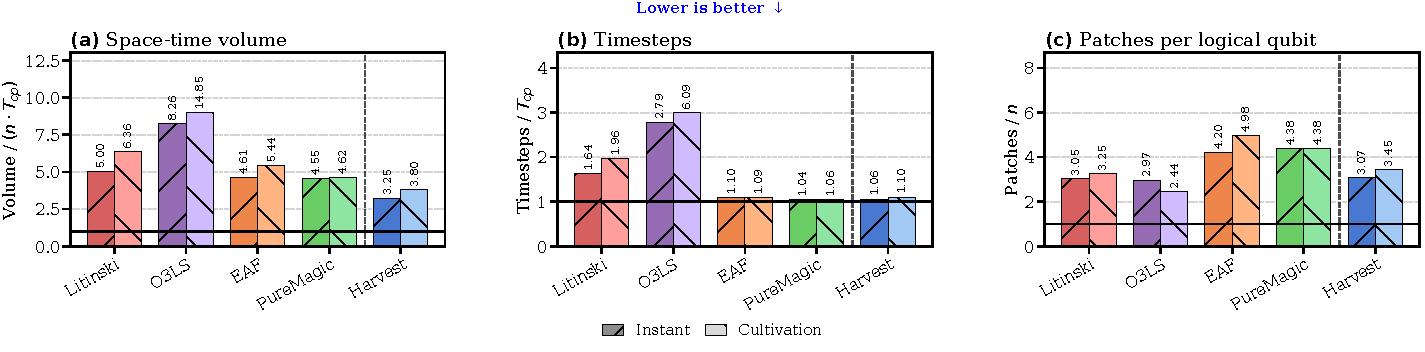
\includegraphics[width=\linewidth]{figures/evaluation/fig_rq1_sota.pdf}
  \caption{\textbf{Comparison with the state of the art} (RQ1). Geometric means over all circuits under instant (dark) and cultivated (light) magic states, normalized to circuit size $n$ and critical-path length $T_{cp}$. \textbf{(a)}~Space--time volume per data patch and critical-path step. \textbf{(b)}~Timesteps over the critical path. \textbf{(c)}~Patches per logical qubit. The solid line marks the respective lower bound: $n$ data patches for $T_{cp}$ steps. Bars above the axis limit are clipped and labeled with their value.}
  \label{fig:rq1-sota}
\end{figure}

% Generated by make_eval_plots.py from rq/rq1_view/rq1_per_circuit.csv
\begin{table}[t]
\centering\small
\caption{Comparison with state-of-the-art lattice-surgery compilers on the 120 (instant) / 120 (cultivation) circuits Harvest has completed (a baseline missing a circuit is left out of that circuit's ratios). Ratios are geometric means of compiler\,/\,Harvest per circuit (lower is better, Harvest $=1$). $T/T_{cp}$: timesteps over the critical-path length. W/T/L: circuits on which Harvest has lower / equal ($\pm$1\%) / higher volume. $T{<}$H: circuits with fewer timesteps than Harvest. Compile time is the geometric mean in seconds; Harvest's includes all four layout templates.}
\label{tab:sota}
\setlength{\tabcolsep}{3.2pt}
\resizebox{\textwidth}{!}{%
\begin{tabular}{l rrrrrrr rrrrrrr}
\toprule
 & \multicolumn{7}{c}{Instant magic states} & \multicolumn{7}{c}{Cultivated magic states} \\
\cmidrule(lr){2-8}\cmidrule(lr){9-15}
Compiler & Vol. & $T$ & Area & $T/T_{cp}$ & W/T/L & $T{<}$H & Time [s] & Vol. & $T$ & Area & $T/T_{cp}$ & W/T/L & $T{<}$H & Time [s] \\
\midrule
Litinski & 1.93 & 1.98 & 0.97 & 2.20 & 93/11/16 & 0 & 0.06 & 2.15 & 2.35 & 0.92 & 2.72 & 117/1/2 & 0 & 0.07 \\
O3LS & 3.35 & 3.37 & 0.99 & 3.74 & 119/1/0 & 0 & 0.98 & 5.29 & 7.51 & 0.70 & 8.70 & 120/0/0 & 0 & 1.13 \\
EAF & 1.41 & 1.06 & 1.32 & 1.18 & 111/3/0 & 14 & 8.62 & 1.42 & 1.00 & 1.42 & 1.09 & 100/2/1 & 46 & 4.26 \\
PureMagic & 1.32 & 0.94 & 1.41 & 1.04 & 105/1/14 & 39 & 0.11 & 1.16 & 0.92 & 1.26 & 1.06 & 90/0/30 & 78 & 0.12 \\
Harvest & \textbf{1.00} & 1.00 & 1.00 & 1.11 & -- & -- & 5.42 & \textbf{1.00} & 1.00 & 1.00 & 1.16 & -- & -- & 5.53 \\
\bottomrule
\end{tabular}}
\end{table}

\begin{figure}[t]
  \centering
  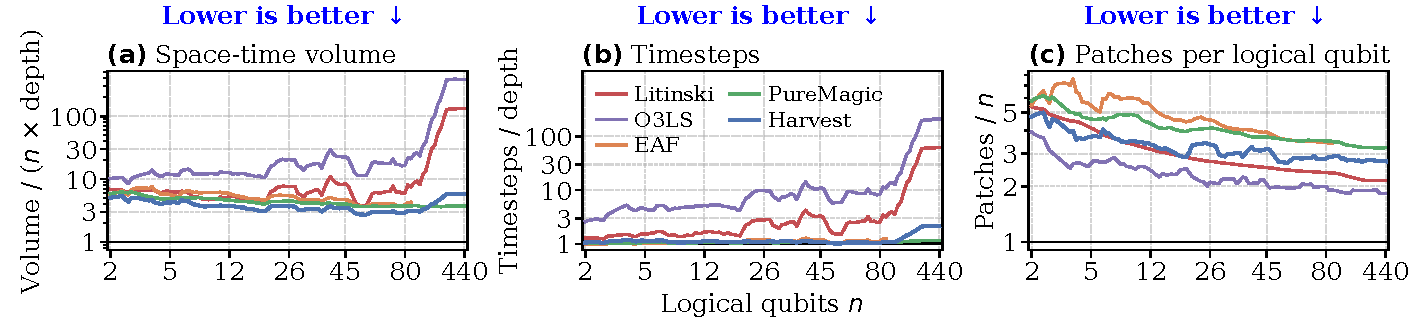
\includegraphics[width=\linewidth]{figures/evaluation/fig_rq1_size_cultivation.pdf}
  \caption{\textbf{Scaling with circuit size} (RQ1), cultivated magic states. Circuits are sorted by the number of logical qubits $n$ (tick labels). \textbf{(a)}~Normalized space--time volume, \textbf{(b)}~timesteps over the circuit depth, and \textbf{(c)}~patches per logical qubit. Lines show the geometric mean over nine neighboring circuits. The solid black line marks the lower bound.}
  \label{fig:rq1-size}
\end{figure}


\myparagraph{Methodology}
We compile every circuit with all five compilers under instant and cultivated supply and compute timesteps, area, and volume.
Fig.~\ref{fig:rq1-sota} reports the size-normalized metrics, Table~\ref{tab:sota} the ratios to Harvest together with per-circuit wins and compile times, and Fig.~\ref{fig:rq1-size} shows how they evolve with circuit size.

\myparagraph{Analysis}
Harvest has the lowest space--time volume under both supply models (Fig.~\ref{fig:rq1-sota}a).
Its normalized volume is 3.25 under instant and 3.80 under cultivated supply, compared with 4.55 and 4.62 for PureMagic, 4.61 and 5.44 for EAF, 5.00 and 6.36 for Litinski, and 8.26 and 14.85 for O3LS.
Per circuit, PureMagic, EAF, Litinski, and O3LS have a larger volume than Harvest by $1.40\times$, $1.42\times$, $1.54\times$, and $2.54\times$ under instant supply and by $1.22\times$, $1.43\times$, $1.67\times$, and $3.90\times$ under cultivated supply (Table~\ref{tab:sota}).
Harvest has the lower volume on 87 of 91 circuits against PureMagic under instant supply and on 73 of 91 under cultivated supply.

The improvement stems from area rather than time.
Harvest, EAF, and PureMagic all schedule within 10\% of the critical path (Fig.~\ref{fig:rq1-sota}b), with PureMagic slightly ahead at $1.04\times$ and $1.06\times$ $T_{cp}$ against $1.06\times$ and $1.10\times$ for Harvest.
Harvest, however, needs only 3.07 and 3.45 patches per logical qubit, whereas EAF and PureMagic need 4.20 to 4.98 (Fig.~\ref{fig:rq1-sota}c).
Litinski and O3LS use layouts as compact as Harvest's but schedule $1.6\times$ to $6.1\times$ longer than the critical path, so their volume is the largest.

The advantage persists as circuits grow (Fig.~\ref{fig:rq1-size}).
For circuits with more than 20 logical qubits, the normalized volume of Harvest stays between 3.3 and 3.5 under cultivated supply, whereas the volume of Litinski and O3LS grows with the circuit size.
Under instant supply, Harvest's timesteps rise slightly to $1.15\times$ $T_{cp}$ for the largest circuits, where PureMagic remains at $1.06\times$.

\statementLeftAccent{Takeaway \#1}{green}{Harvest achieves the lowest space--time volume under both supply models, $1.22$--$3.90\times$ below the other compilers. All three dependency-aware compilers schedule within 10\% of the critical path, and Harvest wins through a smaller layout of about three patches per logical qubit.}

%% ---------------------------------------------------------------------------
\subsection{Sources of the Improvement}
\label{sec:eval-contributions}

\researchquestion[RQ2: Contributions]{Which stages of Harvest account for its lower volume?}

\begin{figure}[t]
  \centering
  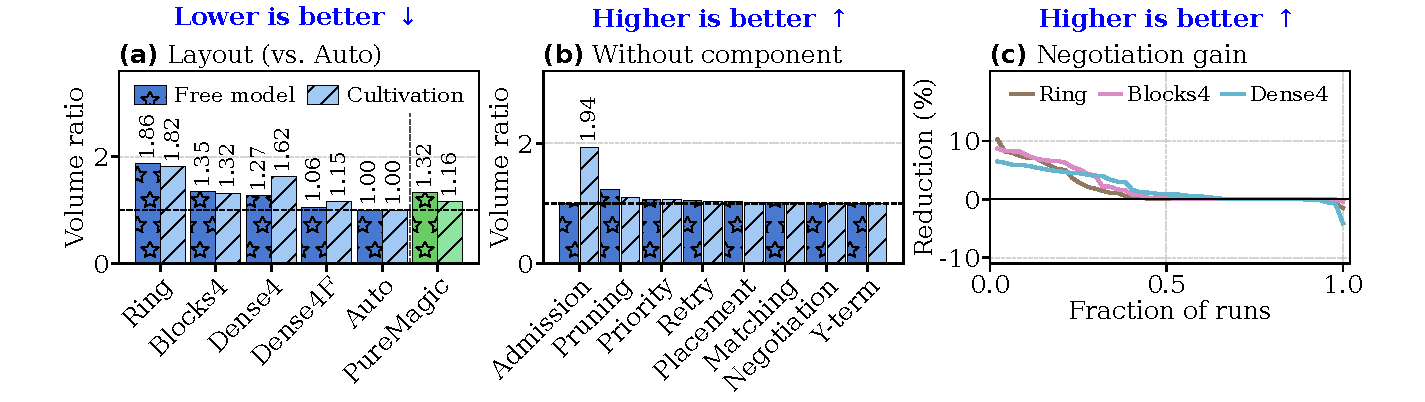
\includegraphics[width=\linewidth]{figures/evaluation/fig_rq2_contributions.pdf}
  \caption{\textbf{Sources of the improvement} (RQ2). \textbf{(a)}~Volume of Harvest restricted to a single layout template, and of PureMagic, relative to Harvest's per-circuit template choice (Auto). \textbf{(b)}~Leave-one-out ablation: volume of Harvest without one component, relative to full Harvest. \textbf{(c)}~Timestep reduction from negotiated-congestion routing per run, sorted, for three templates.}
  \label{fig:rq2-contributions}
\end{figure}


\myparagraph{Methodology}
We first restrict Harvest to a single layout template and compare its volume with the per-circuit choice among all four templates.
We then remove one component at a time on the ring, blocks-of-four, and dense templates: admission control (line~4 of Algorithm~1), pruning, height-based priority, the retry of deferred operations (line~15), circuit-aware placement, terminal selection, negotiated rerouting (lines~10--13), and the $Y$-factor term of the placement cost.
Each variant runs on the 47-circuit subset under instant supply and under cultivated supply with three seeds.

\myparagraph{Analysis}
The choice of layout template has the largest effect (Fig.~\ref{fig:rq2-contributions}a).
Restricted to the ring or blocks-of-four template, Harvest needs $1.9\times$ and $1.4\times$ the volume of its per-circuit choice; on blocks-of-four, it is on par with PureMagic under instant supply and 12\% behind under cultivated supply.
The densest template alone comes within 6\% of the per-circuit choice and still improves over PureMagic by $1.32\times$ and $1.14\times$.
Since every template produces an H-IR program that the same scheduler, pruner, and validator process, exploring several templates requires no change to the rest of the pipeline.

Among the remaining components, admission control matters most under cultivated supply (Fig.~\ref{fig:rq2-contributions}b).
Without it, operations claim terminals that hold no magic state and the volume grows by $1.92\times$; under instant supply every terminal is ready, and admission has no effect.
Pruning reduces the volume by $1.24\times$ and $1.11\times$, height-based priority by $1.06\times$, and the retry of deferred operations by $1.03$--$1.04\times$.
Placement, terminal selection, and the $Y$-factor term each change the volume by at most 3\%.

Negotiated rerouting leaves the geometric-mean volume unchanged but shortens individual schedules (Fig.~\ref{fig:rq2-contributions}c).
It reduces the timesteps in 28--44\% of the runs, by up to 9.7\%, mostly for highly parallel circuits such as Ising models, $k$-nearest neighbors, and swap tests, in which many ready operations compete for the same routing patches.
On sparse templates, routes rarely conflict, and the longer detours that negotiation chooses can keep additional routing patches from being pruned.

\statementLeftAccent{Takeaway \#2}{green}{The volume advantage stems mainly from choosing a compact layout per circuit, pruning, and admitting magic-state operations only when a state is ready. Negotiated rerouting shortens congested schedules by up to 9.7\% but has little effect on average.}

%% ---------------------------------------------------------------------------
\subsection{Layout Provisioning and Pruning}
\label{sec:eval-provisioning}

\researchquestion[RQ3: Provisioning]{How many magic-state patches should the working layout provide, and how much of the overprovisioning does pruning recover?}

\begin{figure}[t]
  \centering
  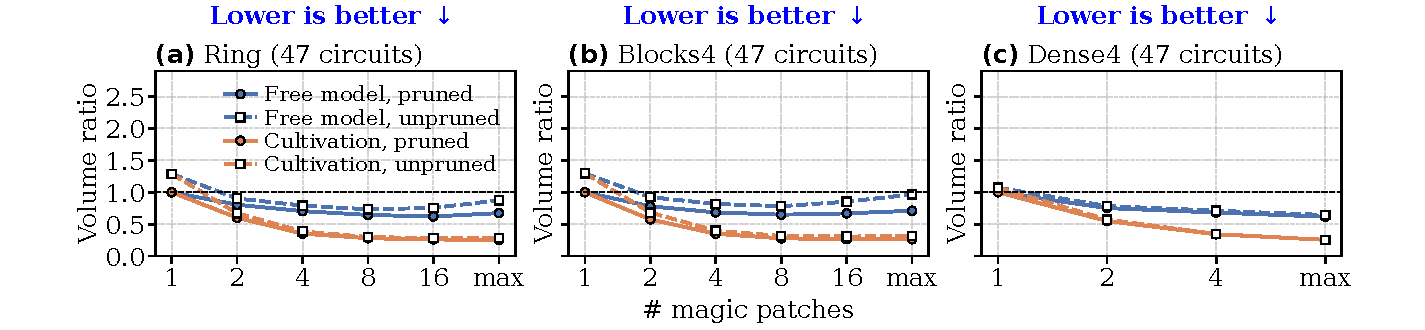
\includegraphics[width=\linewidth]{figures/evaluation/fig_rq3_provisioning.pdf}
  \caption{\textbf{Layout provisioning} (RQ3). Space--time volume as the working layout provides more magic-state patches, relative to the pruned volume with a single magic-state patch, on the \textbf{(a)}~ring, \textbf{(b)}~blocks-of-four, and \textbf{(c)}~dense template. Filled markers show the reported (pruned) volume, open markers the volume of the working layout before pruning. \emph{max} uses every magic-state patch of the template.}
  \label{fig:rq3-provisioning}
\end{figure}


\myparagraph{Methodology}
We vary the number of magic-state patches of the working layout from one to all patches of the template on the ring, blocks-of-four, and dense templates.
For each configuration, we report the volume before and after pruning, relative to the pruned volume with a single magic-state patch, on the 37 circuits that completed every configuration.
To test whether a smaller working layout would have yielded the same schedule, we also reschedule every circuit directly on its pruned layout.

\myparagraph{Analysis}
Under cultivated supply, additional magic-state patches reduce the volume by up to $3.5\times$ (Fig.~\ref{fig:rq3-provisioning}).
The volume drops to 30\% of the single-patch volume at eight patches and stays flat beyond, because every further patch adds area but no longer shortens the schedule.
Under instant supply, additional patches let more rotations run in parallel but also add area, so the volume decreases by at most 29\% and rises again when the working layout provides every magic-state patch of the template.

Pruning makes generous provisioning safe.
Before pruning, the full ring and blocks-of-four layouts exceed the single-patch volume by $1.06\times$ and $1.16\times$ under instant supply.
After pruning, they stay $1.28\times$ and $1.23\times$ below it, since the pruner removes every magic-state and routing patch that the schedule does not use.
Rescheduling directly on the pruned layout yields the same volume (geometric-mean ratio 1.00), so the pruned layout loses no schedule quality.

\statementLeftAccent{Takeaway \#3}{green}{Providing more magic-state patches reduces the volume by up to $3.5\times$ under cultivated supply. Pruning removes the unused patches, so a generously provisioned working layout costs no volume.}

%% ---------------------------------------------------------------------------
\subsection{Magic-State Protocols}
\label{sec:eval-supply}

\researchquestion[RQ4: Supply models]{How close does Harvest come to the lower bound under different magic-state protocols, and what does scheduling against the supply model gain?}

\begin{figure}[t]
  \centering
  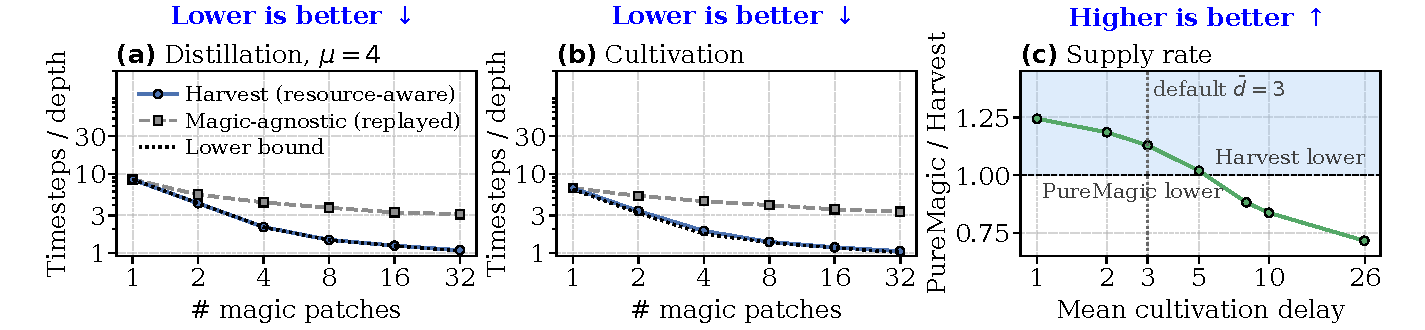
\includegraphics[width=\linewidth]{figures/evaluation/fig_rq4_supply.pdf}
  \caption{\textbf{Magic-state protocols} (RQ4). Timesteps over the critical path as the number of magic-state patches grows under \textbf{(a)}~distillation with $\mu=4$, \textbf{(b)}~distillation with $\mu=10$, and \textbf{(c)}~cultivation. Harvest schedules against the supply model; the magic-oblivious schedule is computed for instant supply and replayed with stalls. The dotted line is the lower bound $\max(T_{cp}, \text{supply})$. Panel titles give the number of circuits.}
  \label{fig:rq4-supply}
\end{figure}

% Generated by make_eval_plots.py from rq/rq4/*.csv
\begin{table}[t]
\centering\small
\caption{Magic-state models behind the \texttt{advance}/\texttt{avail}/\texttt{consume} interface. LoC: lines implementing the interface; no model required changes to the scheduler or validator. All schedules pass (V1)--(V4) before and after pruning. Oblivious: the instant-model schedule replayed under the model; it violates (V4) without stalls, and the ratio gives its stall-inserted timesteps over Harvest's (geometric mean / max). $^\dagger$New in this paper.}
\label{tab:models}
\begin{tabular}{l r c r r r}
\toprule
Model & LoC & Restr.\ stable & Schedules valid & Oblivious invalid & Oblivious / aware \\
\midrule
Instant & 0 & \checkmark & 310/310 & -- & -- \\
Distillation $\mu{=}4$ & 77 & \checkmark & 310/310 & 310/310 & 2.01 / 3.9 \\
Distillation $\mu{=}10$ & 77 & \checkmark & 310/310 & 310/310 & 2.77 / 8.6 \\
Cultivation (exp.) & 125 & \checkmark & 930/930 & 310/310 & 2.26 / 7.4 \\
Cultivation (log-normal)$^\dagger$ & 9 & \checkmark & 930/930 & -- & -- \\
Multiplexed cultivation$^\dagger$ & 52 & \checkmark & 930/930 & -- & -- \\
\bottomrule
\end{tabular}
\end{table}


\myparagraph{Methodology}
We schedule the 47-circuit subset on the ring template with 1 to 32 magic-state patches under distillation with $\mu = 4$ and $\mu = 10$ and under cultivation, using three seeds for stochastic models.
A magic-state protocol bounds the timesteps from below by $\max(T_{cp}, \text{supply})$, where the supply term is the time the given patches need to produce the program's magic states.
As a baseline, we compute each schedule under instant supply and replay it under the target model, inserting a stall whenever a terminal holds no magic state.
We report the 38 circuits that completed every configuration.

\myparagraph{Analysis}
Harvest follows the lower bound under all three protocols (Fig.~\ref{fig:rq4-supply}).
With few magic-state patches, the supply limits the timesteps and Harvest matches the supply bound; with many patches, the timesteps approach the critical path.
In between, Harvest stays within 3\% of the bound under distillation and within 10\% under cultivation.
The magic-oblivious schedules violate (V4) in every case (Table~\ref{tab:models}).
With stalls inserted, they take $2.04\times$, $2.84\times$, and $2.23\times$ longer than Harvest's schedules under distillation with $\mu = 4$, $\mu = 10$, and cultivation, and up to $8.6\times$ longer for individual circuits.
Additional magic-state patches help the oblivious schedules far less: from 4 to 32 patches under distillation with $\mu = 4$, their timesteps drop from $4.1\times$ to $3.0\times$ $T_{cp}$, whereas Harvest's drops from $1.9\times$ to $1.06\times$.

Each protocol enters Harvest only through the functions adv, avail, and cons of \S\ref{sec:model-supply}.
The distillation and cultivation models take 77 and 125 lines, and the log-normal and multiplexed cultivation variants, which we implemented for this paper, take 9 and 52 lines; none of them required changes to the scheduler or the validator (Table~\ref{tab:models}).

\statementLeftAccent{Takeaway \#4}{green}{Scheduling against the supply model keeps Harvest within 10\% of the lower bound under every protocol, whereas replaying a magic-oblivious schedule is $2.0$--$2.8\times$ slower. New protocols require only the three functions of the supply model.}

%% ---------------------------------------------------------------------------
\subsection{Correctness and Compilation Cost}
\label{sec:eval-validity}

\researchquestion[RQ5: Validity and cost]{Are the schedules that Harvest reports valid, does the validator detect invalid schedules, and how long does compilation take?}

% Generated by make_eval_plots.py from rq/rq5/rq5_census.csv and rq/rq5/rq5_faults.csv
% TODO: census lists 19492 schedules but only 17942 were checked (difference: RQ4 rows) -- confirm these are the oblivious replays.
% TODO: fault descriptions are inferred from the fault names -- check against the injector.
% NOTE: the per-rule labels in rq5_faults.csv look swapped (V2<->V3); rules are omitted until checked.
\begin{table}[t]
\centering\small
\caption{Validator results. 17,942 Harvest schedules from RQ1--RQ5 were checked against (V1)--(V4) before and after pruning, with 0 violations. Below: injected scheduler faults and random schedule corruptions; applicable runs are those in which the fault changes the schedule.}
\label{tab:validity}
\begin{tabular}{ll rr rr}
\toprule
 & & \multicolumn{2}{c}{Instant} & \multicolumn{2}{c}{Cultivation} \\
\cmidrule(lr){3-4}\cmidrule(lr){5-6}
Study & Fault & Applicable & Caught & Applicable & Caught \\
\midrule
Scheduler bug & Drop a port of a $Y$ factor & 43 & 100\% & 43 & 100\% \\
 & Consume a state before it is ready & 0 & n/a & 38 & 100\% \\
 & Commit conflicting routes & 36 & 100\% & 38 & 100\% \\
 & Prune a used tile & 47 & 100\% & 47 & 100\% \\
 & Reuse a magic terminal & 46 & 100\% & 46 & 100\% \\
 & Schedule before a predecessor & 47 & 100\% & 47 & 100\% \\
\midrule
Corruption & Disconnect a route & 940 & 100\% & 940 & 100\% \\
 & Drop a dependency & 940 & 100\% & 940 & 100\% \\
 & Overlap two routes & 920 & 100\% & 920 & 100\% \\
 & Use an unavailable state & 0 & n/a & 940 & 100\% \\
\bottomrule
\end{tabular}
\end{table}

\begin{figure}[t]
  \centering
  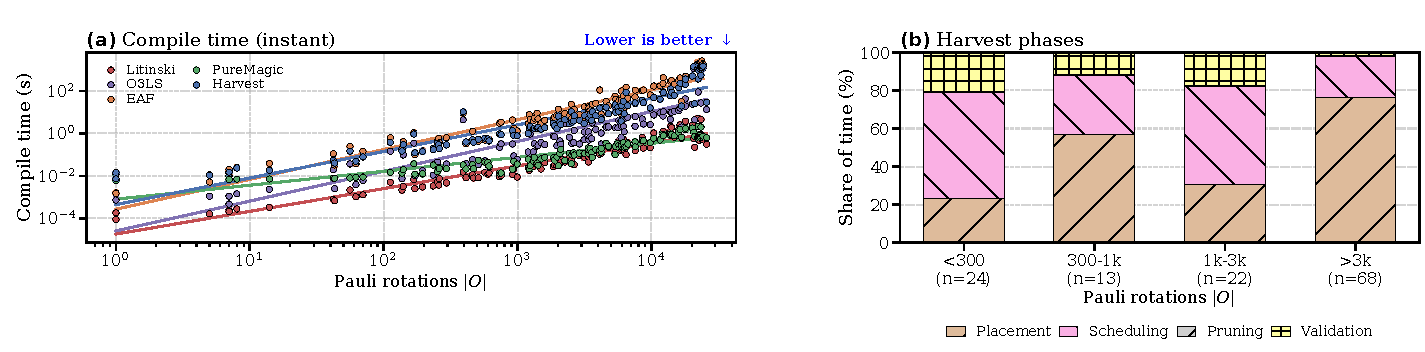
\includegraphics[width=\linewidth]{figures/evaluation/fig_rq5_compile.pdf}
  \caption{\textbf{Compilation cost} (RQ5). \textbf{(a)}~Compile time over the number of Pauli rotations under instant magic states, with log--log fits; Harvest's time includes all four layout templates. \textbf{(b)}~Share of Harvest's compile time per stage, by circuit size.}
  \label{fig:rq5-compile}
\end{figure}


\myparagraph{Methodology}
We validate every Harvest schedule of RQ1--RQ4 before and after pruning.
To test the validator itself, we inject six faults into the scheduler, such as committing conflicting routes or consuming a magic state before it is ready, and apply four kinds of random corruption to valid schedules, 20 per circuit and kind, on the 47-circuit subset.
We measure compile time for all compilers under instant supply.

\myparagraph{Analysis}
All 15{,}213 Harvest schedules satisfy (V1)--(V4) before and after pruning \jannik{confirm the 1{,}305 unchecked RQ4 rows are the oblivious replays}.
The validator detects every injected fault and every corruption that changes the schedule (Table~\ref{tab:validity}).
Validation takes 3--22\% of the compile time.

Harvest compiles a circuit in 1.5\,s in the geometric mean, including all four templates, compared with 2.7\,s for EAF, 0.23\,s for O3LS, 0.06\,s for PureMagic, and 0.02\,s for Litinski (Fig.~\ref{fig:rq5-compile}a).
The compile time grows linearly with the number of rotations overall and with an exponent of 1.44 for circuits with more than 1{,}000 rotations.
Scheduling and placement dominate the compile time, and pruning is negligible (Fig.~\ref{fig:rq5-compile}b).

\statementLeftAccent{Takeaway \#5}{green}{Every one of the 15{,}213 reported schedules is valid on its pruned layout, and the validator catches every injected fault. Harvest compiles a circuit in 1.5\,s on average, with near-linear scaling in the number of rotations.}
